\documentclass[sigconf]{acmart}

\usepackage{booktabs} % For formal tables
\usepackage{amsmath}
\usepackage{multirow}
\usepackage{hyperref}
\usepackage{subcaption}

\DeclareMathAlphabet\mathbfcal{OMS}{cmsy}{b}{n}

\newcommand{\cmt}[1]{\textbf{\textcolor{red}{#1}}}

\renewcommand\footnotetextcopyrightpermission[1]{} % removes footnote with conference information in first column
\settopmatter{printacmref=false}
\pagestyle{plain} % removes running headers

% Copyright
\setcopyright{none}
%\setcopyright{acmcopyright}
%\setcopyright{acmlicensed}
% \setcopyright{rightsretained}
%\setcopyright{usgov}
%\setcopyright{usgovmixed}
%\setcopyright{cagov}
%\setcopyright{cagovmixed}


% DOI
% \acmDOI{10.475/123_4}

% ISBN
% \acmISBN{123-4567-24-567/08/06}

%Conference
% \acmConference[WOODSTOCK'97]{ACM Woodstock conference}{July 1997}{El
%   Paso, Texas USA}
% \acmYear{1997}
% \copyrightyear{2016}


% \acmArticle{4}
% \acmPrice{15.00}

% These commands are optional
%\acmBooktitle{Transactions of the ACM Woodstock conference}
% \editor{Jennifer B. Sartor}
% \editor{Theo D'Hondt}
% \editor{Wolfgang De Meuter}


\hypersetup{draft}
\begin{document}
\title{DeepJIT: An End-To-End Deep Learning Framework for Just-In-Time Defect Prediction}
% \titlenote{Produces the permission block, and
%   copyright information}
% \subtitle{Extended Abstract}
% \subtitlenote{The full version of the author's guide is available as
%   \texttt{acmart.pdf} document}

\author{\IEEEauthorblockN{Thong Hoang\textsuperscript{1}, Hoa Khanh Dam\textsuperscript{2}, Yasutaka Kamei\textsuperscript{3}, David Lo\textsuperscript{1}, Naoyasu Ubayashi\textsuperscript{3}},  \\
\IEEEauthorblockA{\textsuperscript{1}Singapore Management University, Singapore\\ \textsuperscript{2}University of Wollongong, Australia\\
\textsuperscript{3}Kyushu University, Japan} \\ 
vdthoang.2016@smu.edu.sg, hoa@uow.edu.au, kamei@ait.kyushu-u.ac.jp, \\ davidlo@smu.edu.sg, ubayashi@ait.kyushu-u.ac.jp
}

% \author{Thong Hoang, David Lo}
% \affiliation{%
%   \institution{Singapore Management University, Singapore}
% }
% \email{{vdthoang.2016, davidlo}@smu.edu.sg}

% \author{Hoa Khanh Dam}
% \affiliation{%
%   \institution{University of Wollongong, Australia}
% }
% \email{hoa@uow.edu.au}

% \author{Yasutaka Kamei, Naoyasu Ubayashi}
% \affiliation{%
%   \institution{Kyushu University, Japan}
% }
% \email{{kamei, ubayashi}@ait.kyushu-u.ac.jp}

% \author{Valerie B\'eranger}
% \affiliation{%
%   \institution{Inria Paris-Rocquencourt}
%   \city{Rocquencourt}
%   \country{France}
% }
% \author{Aparna Patel}
% \affiliation{%
%  \institution{Rajiv Gandhi University}
%  \streetaddress{Rono-Hills}
%  \city{Doimukh}
%  \state{Arunachal Pradesh}
%  \country{India}}
% \author{Huifen Chan}
% \affiliation{%
%   \institution{Tsinghua University}
%   \streetaddress{30 Shuangqing Rd}
%   \city{Haidian Qu}
%   \state{Beijing Shi}
%   \country{China}
% }

% \author{Charles Palmer}
% \affiliation{%
%   \institution{Palmer Research Laboratories}
%   \streetaddress{8600 Datapoint Drive}
%   \city{San Antonio}
%   \state{Texas}
%   \postcode{78229}}
% \email{cpalmer@prl.com}

% \author{John Smith}
% \affiliation{\institution{The Th{\o}rv{\"a}ld Group}}
% \email{jsmith@affiliation.org}

% \author{Julius P.~Kumquat}
% \affiliation{\institution{The Kumquat Consortium}}
% \email{jpkumquat@consortium.net}

% % The default list of authors is too long for headers.
% \renewcommand{\shortauthors}{B. Trovato et al.}

%
% The code below should be generated by the tool at
% http://dl.acm.org/ccs.cfm
% Please copy and paste the code instead of the example below.
%
% \begin{CCSXML}
% <ccs2012>
%  <concept>
%   <concept_id>10010520.10010553.10010562</concept_id>
%   <concept_desc>Computer systems organization~Embedded systems</concept_desc>
%   <concept_significance>500</concept_significance>
%  </concept>
%  <concept>
%   <concept_id>10010520.10010575.10010755</concept_id>
%   <concept_desc>Computer systems organization~Redundancy</concept_desc>
%   <concept_significance>300</concept_significance>
%  </concept>
%  <concept>
%   <concept_id>10010520.10010553.10010554</concept_id>
%   <concept_desc>Computer systems organization~Robotics</concept_desc>
%   <concept_significance>100</concept_significance>
%  </concept>
%  <concept>
%   <concept_id>10003033.10003083.10003095</concept_id>
%   <concept_desc>Networks~Network reliability</concept_desc>
%   <concept_significance>100</concept_significance>
%  </concept>
% </ccs2012>
% \end{CCSXML}

% \ccsdesc[500]{Computer systems organization~Embedded systems}
% \ccsdesc[300]{Computer systems organization~Redundancy}
% \ccsdesc{Computer systems organization~Robotics}
% \ccsdesc[100]{Networks~Network reliability}


% \keywords{ACM proceedings, \LaTeX, text tagging}

\begin{abstract}
Most software Quality Assurance (SOA) resources often focus on software modules that are likely to be defective in the future to help developers saving their effort to debug a program. To solve this problem, change-level defect prediction or Just-in-time (JIT) defect prediction is proposed to identify bug in the code changes. JIT models are trained using machine learning techniques which assume that historical changes are similar to future one. Hence, these changes can be used to identify defect-prone software modules (e.g., functions, files, system, etc.). A previous approach relies on manually extracted code changes features. This approach, however, shows only moderate accuracy. In this paper, we propose a novel deep learning framework that is automatically extracting features from commit message and code changes and using them to identify bugs. Our framework takes into account the hierarchical structure of code changes to produce their features. Experiments on two well-known projects (i.e., QT and OPENSTACK) shows that our proposed approach outperforms the state-of-the-art baseline in term of the area under the receiver operator characteristics Curve (AUC). 
\end{abstract}
\maketitle
\section{Introduction}

As software systems are becoming the backbone of our economy and society, defects existing in those systems may substantially affect businesses and people's lives  in many ways. For example, Knight Capital\footnote{https://dealbook.nytimes.com/2012/08/02/knight-capital-says-trading-mishap-cost-it-440-million/}, a company which executes automated trading  for retail brokers, lost \$440 millions in only one morning in 2012 due to an overnight faulty update to its trading software. A flawed code change, introduced into OpenSSL's source code repository, caused the infamous Heartbleed\footnote{http://heartbleed.com} bug which affected billions of Internet users in 2014. As software grows significantly in both size and complexity, finding defects and fixing them become increasingly difficult and costly.

One common best practice for cost saving is identifying defects and fixing them as early as possible, ideally before new code changes (i.e. \emph{commits}) are introduced into codebases. Emerging research has thus developed \emph{Just-In-Time} (JIT) defect prediction models and techniques which help software engineers and testers to quickly narrow down the most likely defective commits to a software codebase  \cite{KameiS16,D'Ambros:2012:EDP}. JIT defect prediction tools helps provide early feedback to software developer, and prioritize and optimize effort for inspection and (regression) testing, especially when facing with deadlines and limited resources. They have therefore been integrated into the development practice at large software organizations such as Avaya \cite{Mockus2000}, Blackberry \cite{Shihab:2012:ISR}, and Cisco \cite{Tantithamthavorn:2015:IMP}.

Machine learning techniques have been widely used in existing work for building JIT defect prediction models. A common theme of existing work (e.g. \cite{Kamei:2013:LES,Kim:2008:CSC,Kononenko:2015,Mockus2000,McIntosh:2018:FCM}) is carefully crafting a set of features representing a code change, and using them as defectiveness predictors. Those features are mostly derived from the properties of code changes, such as the change size (e.g. lines added or deleted), the change scope (e.g. the number of files or directories modified), the history of changes (e.g. the number of prior changes to the updated files), track record of the author and code reviewers, and the activeness of the code review of the change. Those features are then used by a traditional classifier (e.g. Random Forests or Logistic Regression) to predict the defectiveness of code changes A recent work \cite{Yang:2015:DLJ}  used a deep learning model (i.e. Deep Belief Network) to improve the performance of JIT defect prediction models. Their approach does not, however, leverage the true notions of deep learning. They still used the same set of features that are manually engineered as in previous work, and their model is \emph{not} end-to-end trainable.

The metric-based features however do not represent the semantic and syntactical structure of the actual code changes. In many cases, two different code changes which have the exactly same metrics (e.g. the number of lines added and deleted) may generate different behaviour when executed, and thus have a different likelihood of defectiveness. Previous studies have showed the usefulness of harvesting the syntactical structure and semantic information hidden in source code to perform various software engineering tasks such as code completion, bug detection and defect prediction \cite{Wang:2016:ALS,Tu:2014:LS,Nguyen:2015:GSL,Hindle:2012:NS,Li:2005:PAE}. This information may enrich representations for defective code changes, and thus improve JIT defect prediction.

In this paper, we present a new JIT defect prediction model (namely DeepJIT) which leverages the powerful deep learning Convolution Neural Network (CNN) architecture to learn a deep representation of commits. Our model processes both a commit message (in natural language) and the associated code changes (in programming languages) and automatically semantic features which represent the ``meaning'' of the commit. This approach removes software practitioners from manually designing and extracting features, as done in previous work. DeepJIT is a fully end-to-end trainable system where raw data signals (e.g. words or code tokens) are passed from input nodes up to the final output node for predicting defectiveness, and prediction errors are back propagated from the output node down to the input layer.
TODOXXX: Results are summarized here .... 
\begin{figure}[ht]
\center
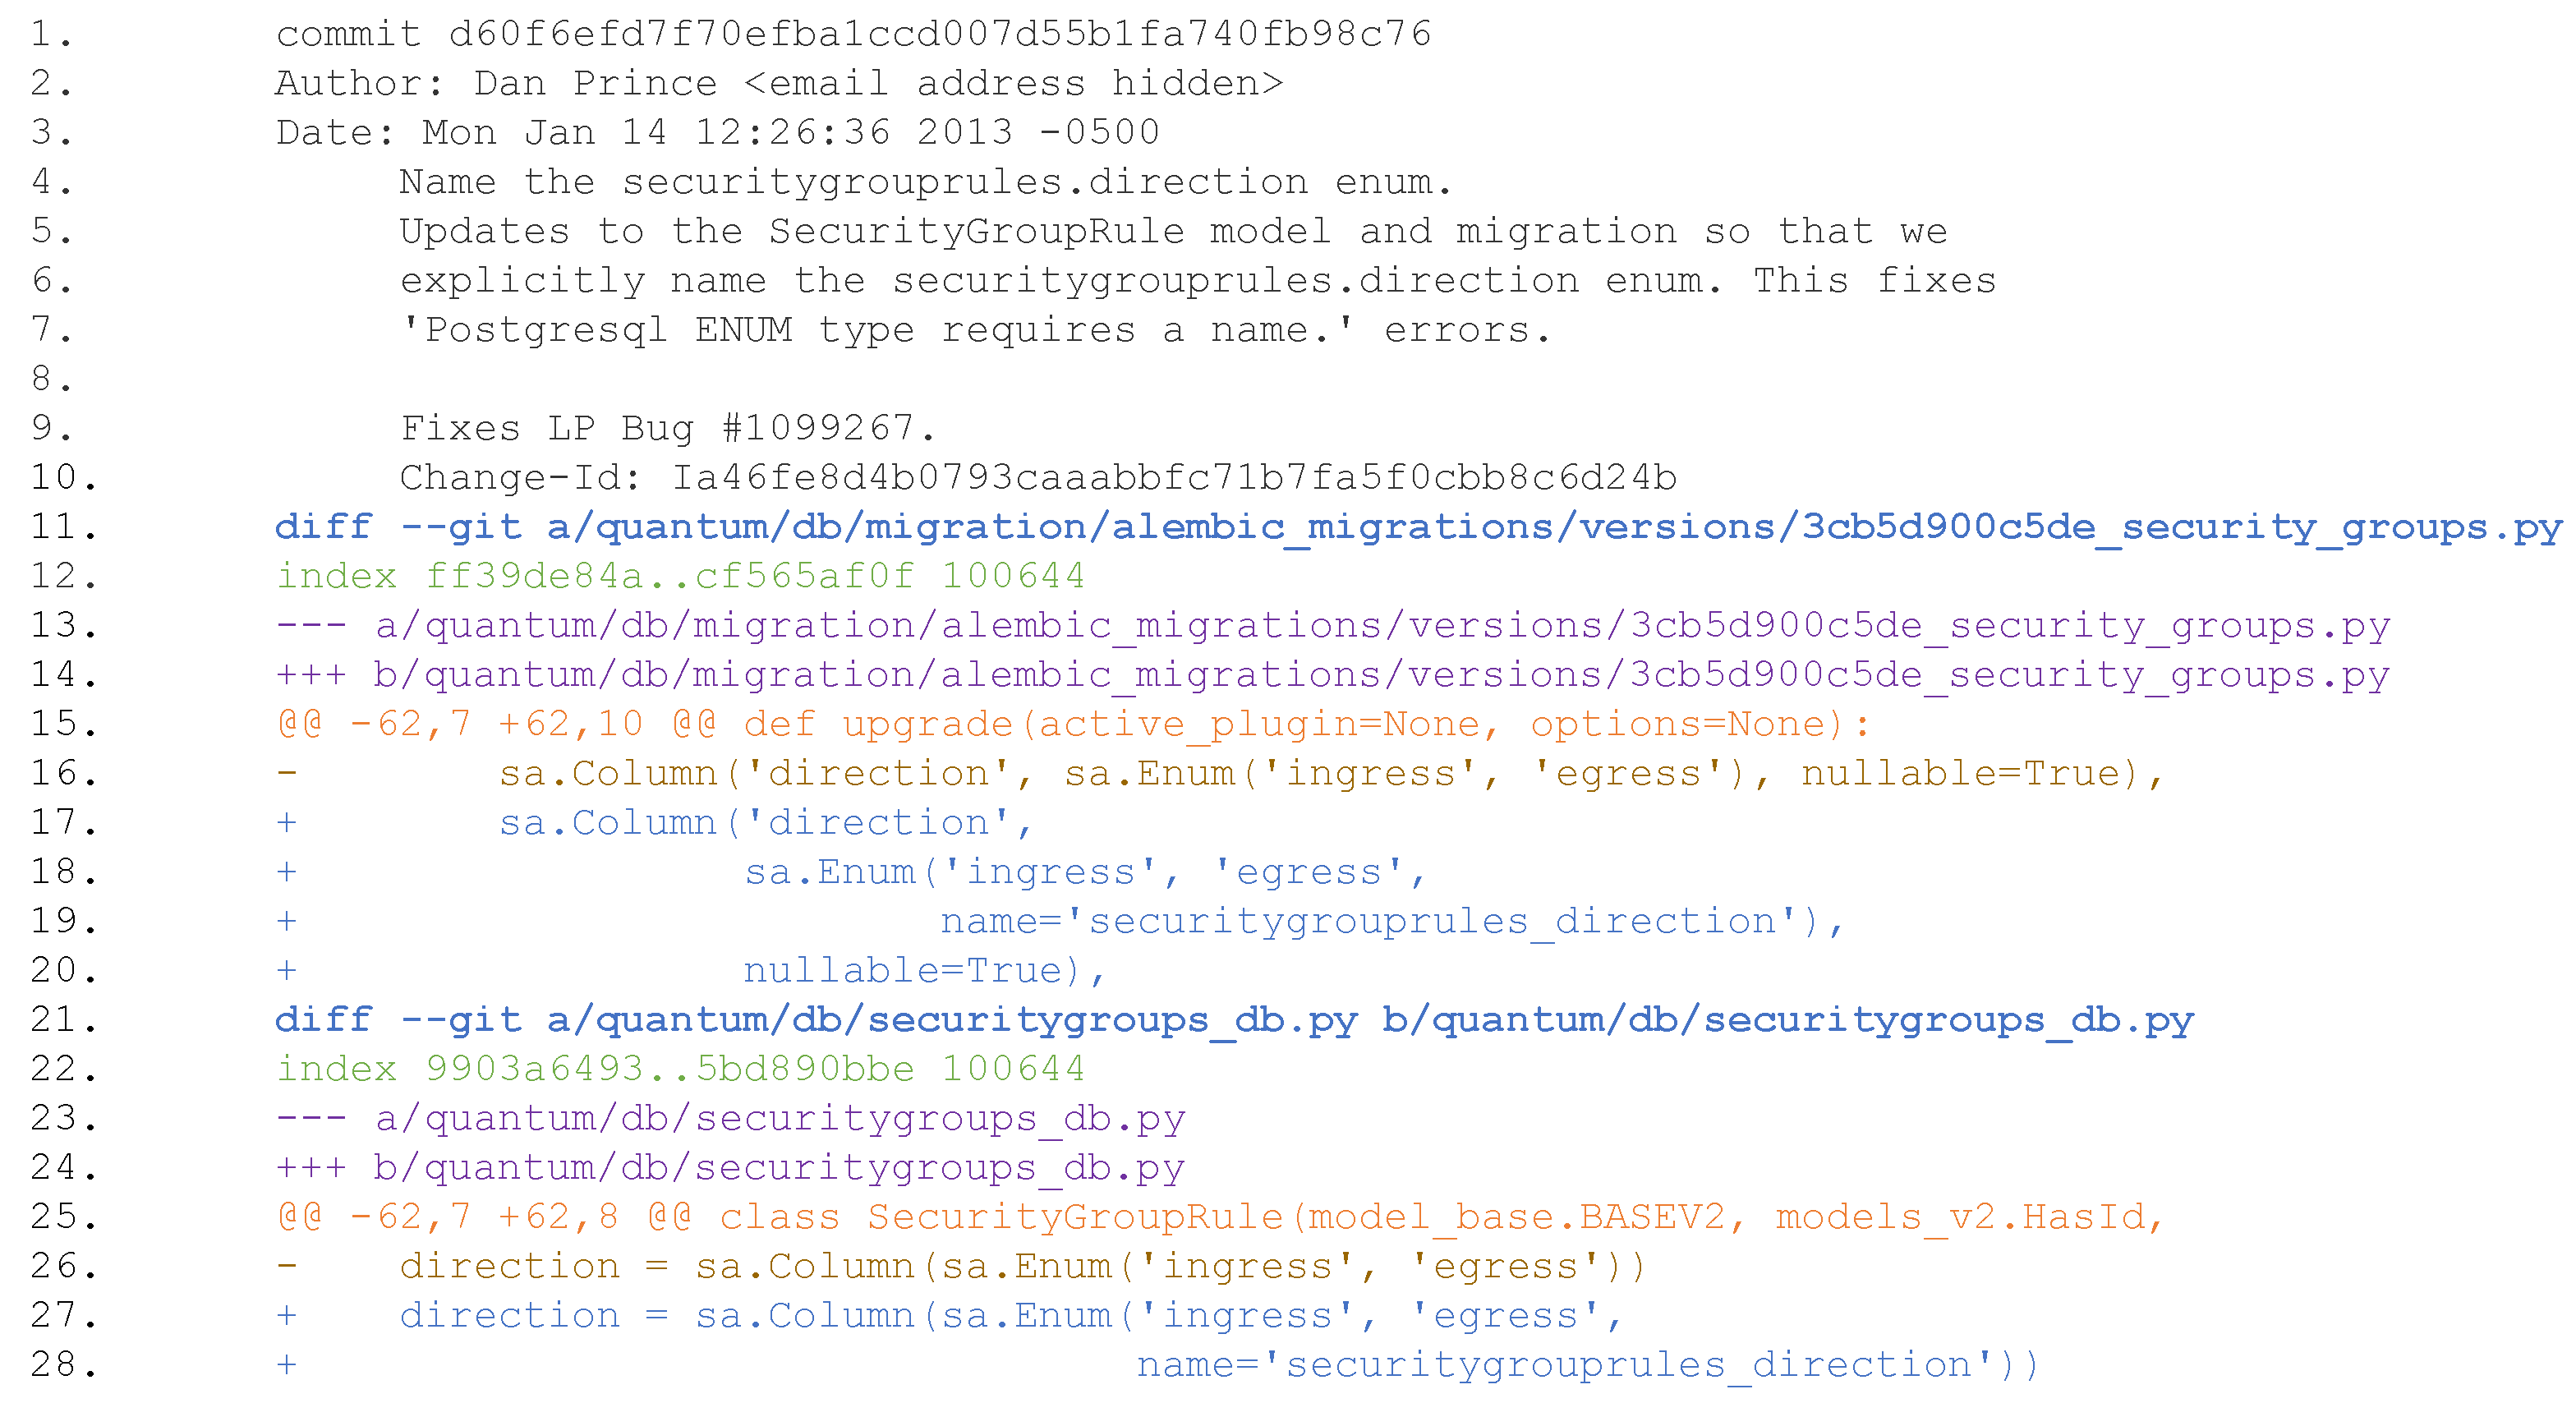
\includegraphics[scale=0.19]{figs/example.pdf}
\caption{An example of a buggy commit change.}
\label{fig:example}
\end{figure} 

\section{Background}
\label{sec:background}

We first present an example of commit change motivating our deep learning framework. We then briefly introduce a background knowledge about Convolutional Neural Network (CNN) used to extract features in the commit change. 

\subsection{Code changes}\label{sec:examle}

Figure~\ref{fig:example} shows a sample of a buggy commit. The buggy commit contains many pieces of information, i.e., a commit id (line 1), a author name (line 2), a commit date (line 3), a commit message (line 4-10) and a set of code changes (i.e., 11-28). The commit message plays an important role when you commit your change since it is the first thing people will see about the change. A good commit message can help maintainers to speed up the reviewing process and write a good release note. A set of code changes includes changes of multiple files and each file includes a number of deleted and added lines representing the change. In the Figure~\ref{fig:example}, line 16 (starting with \texttt{-}) and line 17-20 (starting with \texttt{+}) indicates the deleted and added lines of a change file (namely \texttt{3cb5d900c5de\_security\_groups.py}), respectively. 

Previous works mainly depend on a set of manually features extracted from code changes~\cite{Yang:2015:DLJ, mcintosh2018fix}, however, the manual code features might overlook features which find helpful to identify a buggy commit. Moreover, the commit message in the commit is also ignored. Thus, a powerful feature representation of commit message and code changes is needed to detect buggy commits. 

Inspired by a deep learning Convolutional Neural Network (CNN)~\cite{lecun2015deep}, our deep learning \emph{Just-In-Time} (JIT) defect prediction model (DeepJIT) aims to automatically extract features of the commit message and the code changes of a given commit, respectively. These features are then combined to evaluate whether the given commit is buggy. 
% The key challenge here is to capture the semantic and syntactical structure of the code changes in the given commit. 
Different from the commit message, the code changes include a number of deleted and added lines across multiple files (see Figure~\ref{fig:example}). To solve this problem, we first learn the semantic features of each added or deleted line for each changed file using CNN framework, the semantic features of the added and deleted lines are then incorporated to build a new representation 
% preserving the syntactical structure 
of the change file. We again use CNN to extract features from the new representation of the change file. These features of all the change files are used to construct the features of the code changes in the given commit. Section~\ref{sec:approach} briefly describes DeepJIT. 

\subsection{Convolutional Neural Network}
\label{sec:background_cnn}

\begin{figure*}[t!]
	\center
	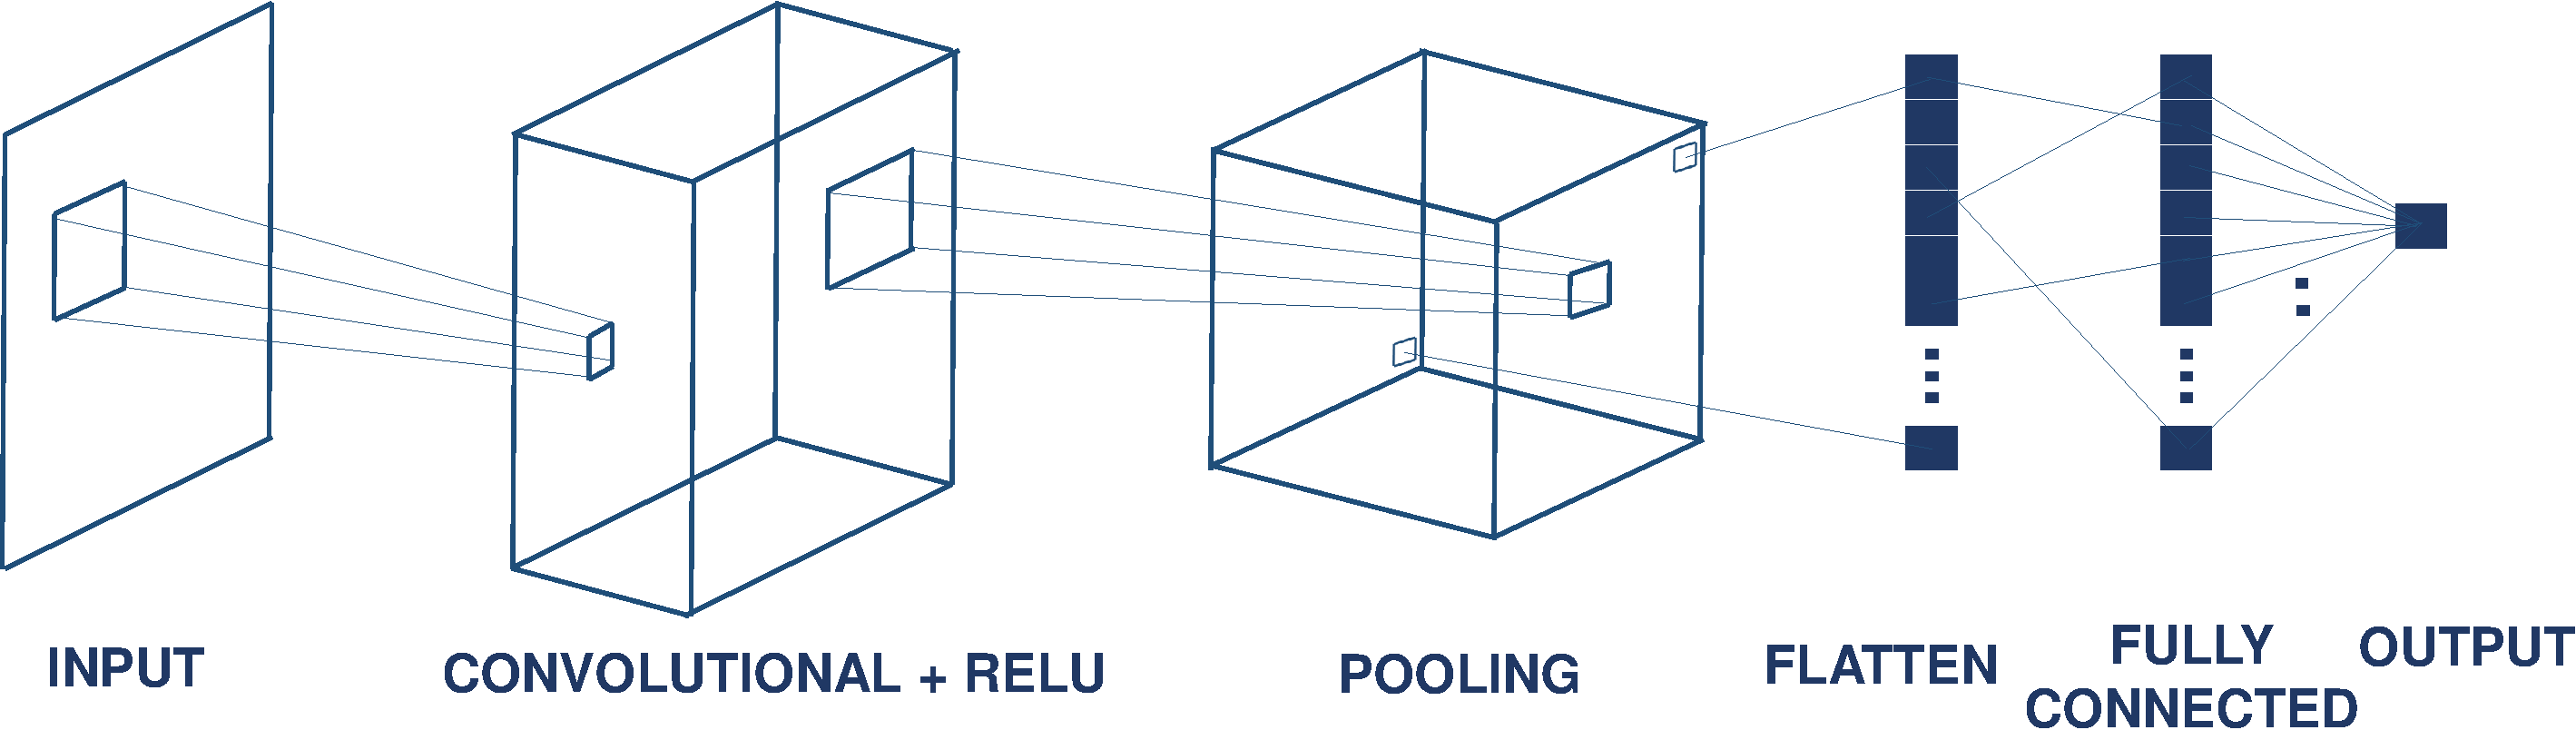
\includegraphics[scale=0.3]{figs/cnn.pdf}
	\caption{A simple convolutional neural network architecture.}
	\label{fig:cnn}
\end{figure*}

\begin{figure*}[t!]
	\center
	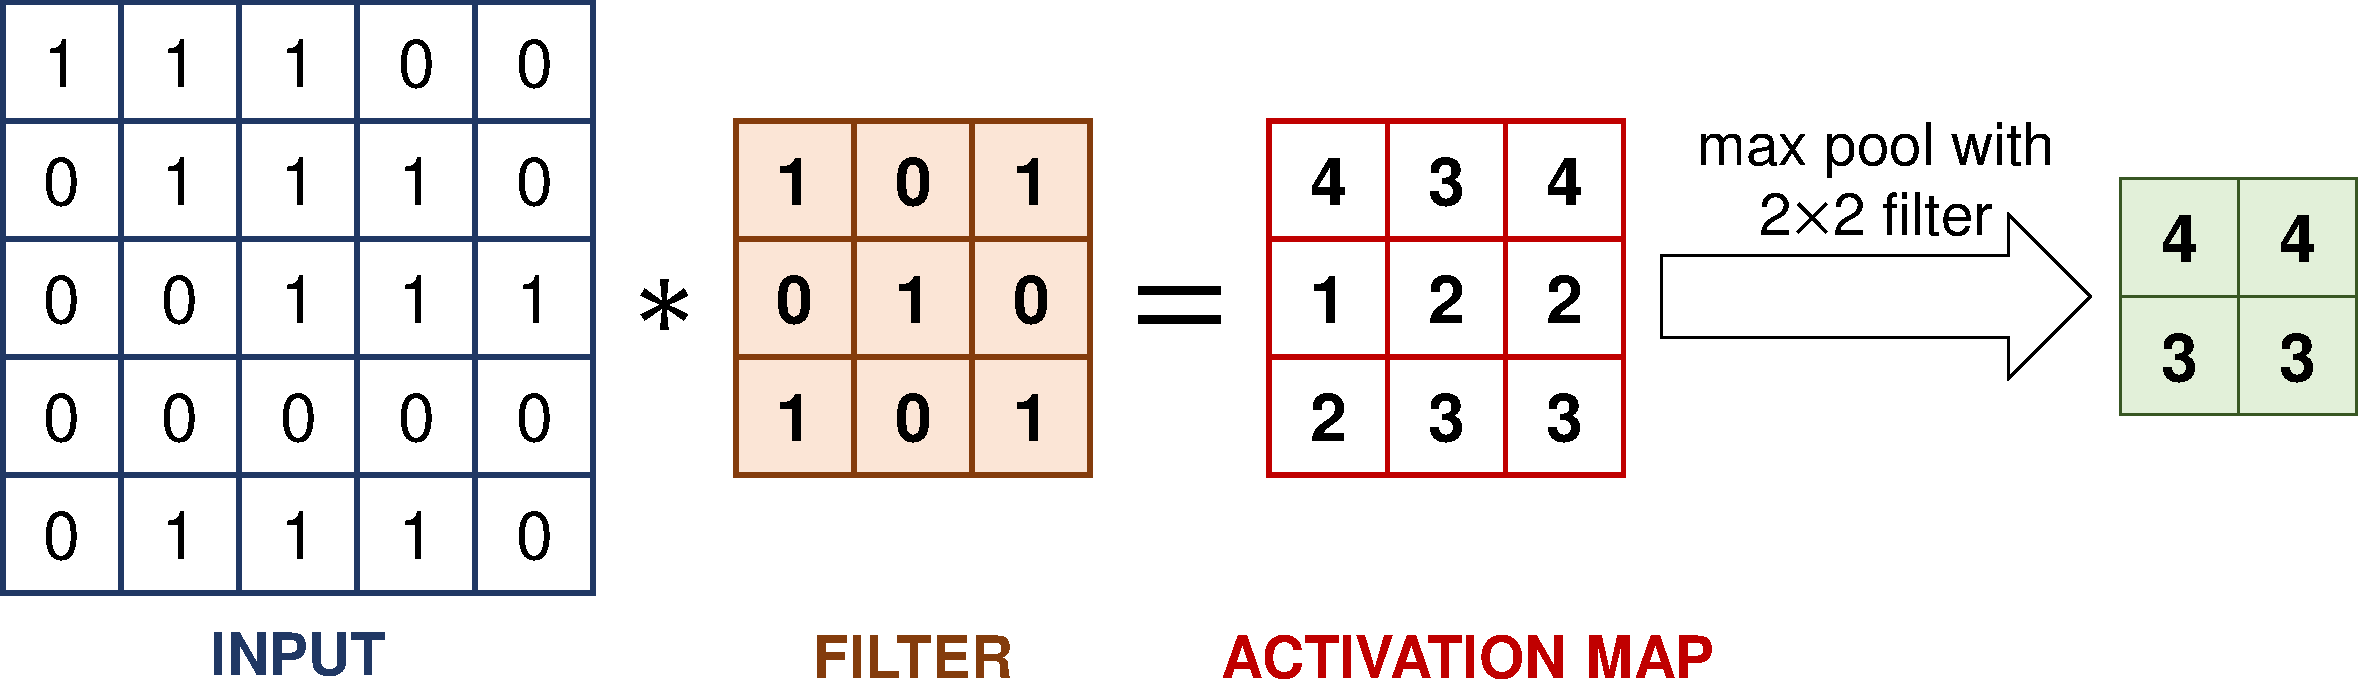
\includegraphics[scale=0.3]{figs/filter_pooling.pdf}
	\caption{An example of a convolutional layer and pooling layer in CNN.}
	\label{fig:filter}
\end{figure*}

One of the most powerful forms of deep learning neural networks is the Convolutional Neural Network (CNN)~\cite{lecun2015deep}. CNNs are widely used to solve image pattern recognition problems and have been achieved significant results~\cite{karpathy2014large, lawrence1997face, krizhevsky2012imagenet}. Like traditional deep learning networks, CNNs receive an input and perform a product operation followed by a nonlinear function. The last layer is the output layer containing objective functions~\cite{zhao2017loss} associated with the labels of the input.

Figure~\ref{fig:cnn} illustrates a simple CNN for classification task. The simple CNN includes an input layer, a convolutional layer, followed by the rectified linear unit (RELU) which is a nonlinear activation function, a pooling layer, a fully-connected layer, and an output layer. We briefly explain these layers in the following paragraphs. 

The input layer takes an input as 2-dimensional array or 3-dimensional array and passes it through a of convolution layers.

The convolutional layer plays a vital role in CNN and it takes advantage of the use of learnable filters. These filters are small in spatial dimensionality, but they are applied along the entirety of the depth of the input data. For example, given an input data $\textbf{I} \in \mathbb{R}^{\text{H} \times \text{W} \times \text{D}}$ and a filter $\textbf{K} \in \mathbb{R}^{\text{h} \times \text{w} \times \text{D}}$, we produce a new activation map $\textbf{A} \in \mathbb{R}^{(\text{H} - \text{h}) \times (\text{W} - \text{w}) \times 1}$. The RELU is then applied to each value of the activation map as follows:
\begin{equation}
\label{eq:relu}
f(x) = max(0, x)   
\end{equation}

The pooling layer, which is an important component of CNN, aims to reduce the dimensionality of the activation map, the number of parameters, and the computational helping to control overfitting problem~\cite{tolias2015particular}. The pooling layer spreads along the activation map and scales its dimensionality. There are three different types of pooling layers:
\begin{itemize}
	\item Max pooling takes the largest element from each region of the activation map.
	\item Average pooling constructs the average value from each region of the activation map.
	\item Sum pooling sums all the elements from each region of the activation map. 
\end{itemize}
In practice, max pooling often achieves a better performance compared to the other two pooling techniques~\cite{zeiler2013stochastic}. Figure~\ref{fig:filter} presents a visual representation of a convolutional layer and pooling layer in CNN. Given an input 5$\times$5 and a filter 3$\times$3, we output a new activation map 3$\times$3. A max pooling layer with a filter 2$\times$2 is then applied to produce a new output. 

The output of pooling layer is flatten and directly passed to a fully connected layer (or a hidden layer). The fully connected layer is passed to an output layer to calculate an objective function (or a loss function)~\cite{zhao2017loss}. The objective function normally is optimized using a stochastic gradient descent (SGD)~\cite{bottou2010large}. This is an analogous way with traditional neural networks~\cite{huang1988neural}.




\section{approach}
\label{sec:approach}
In this section, we first formulate the \emph{Just-In-Time} (JIT) defect prediction problem and provide an overview of our framework. We then describe the details of each part inside the framework. Finally, we present an algorithm for learning effective settings of our model's parameters. 
\subsection{Framework Overview}
\label{sec:overview}

\begin{figure}
\center
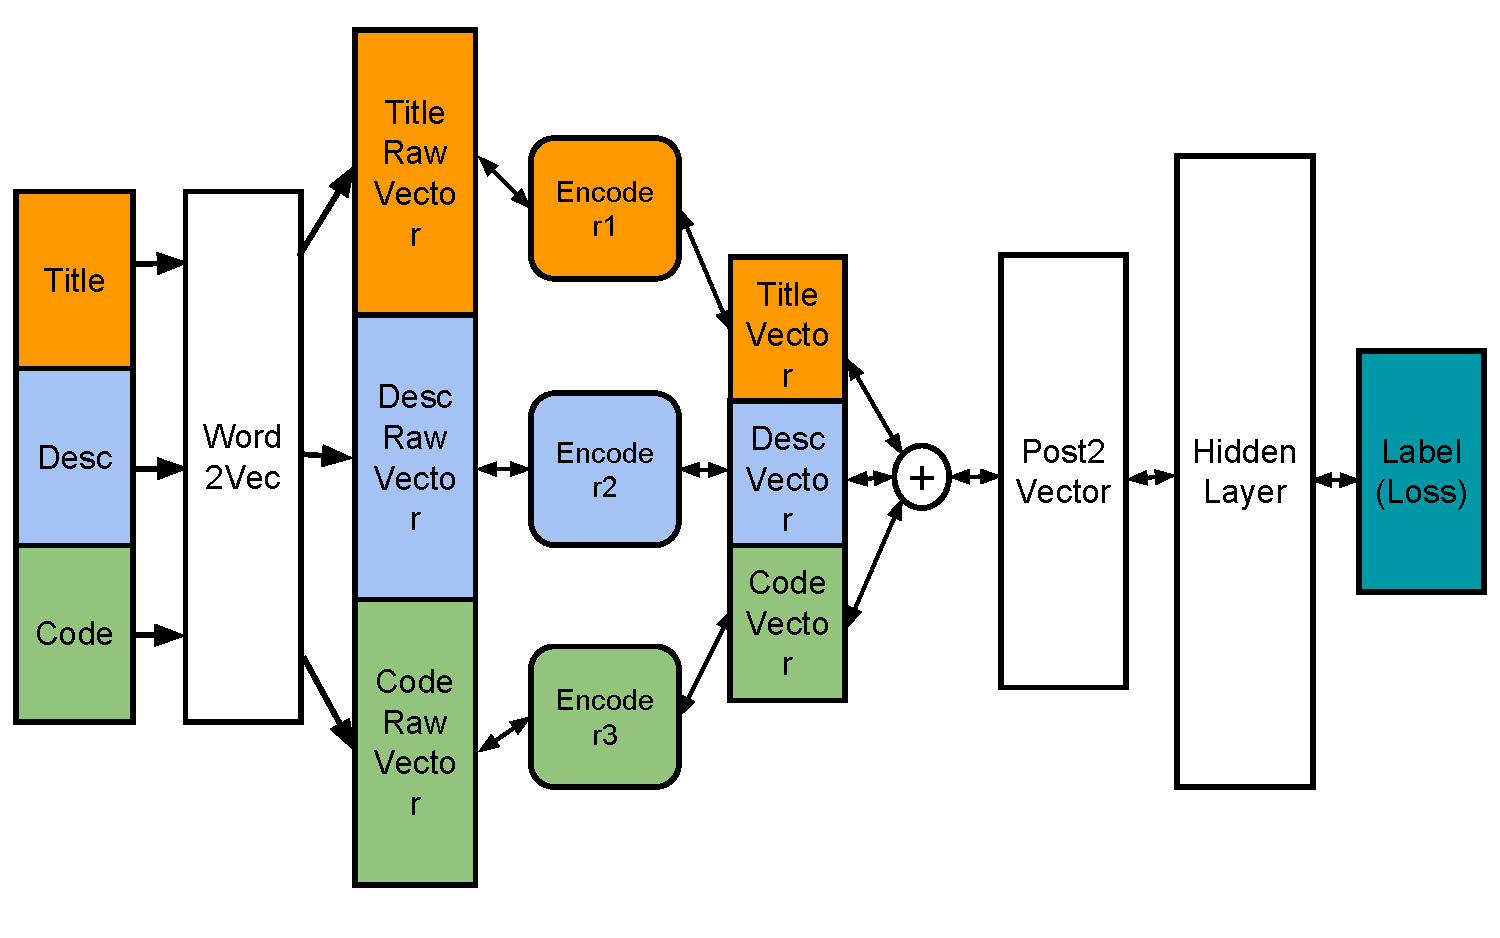
\includegraphics[scale=0.36]{figs/framework.pdf}
\caption{The general framework of just-in-time defect prediction model.}
\label{fig:overview}
\end{figure}

The goal of the just-in-time defect prediction model is to automatically label a commit change as buggy or clean to help developers better focus on their efforts on assuring software quality. We consider the just-in-time defect prediction problem as a learning task to construct prediction function $\textbf{f}:
\mathcal{X} \longmapsto \mathcal{Y}$, where $y_i \in \mathcal{Y} = \{0, 1\}$ indicates whether a commit change $x_i \in \mathcal{X}$ cleans ($y_i = 0$) or contains a buggy code ($y_i = 1$). The prediction function $\textbf{f}$ can be learned by minimizing the following objective function:
\begin{equation}
\underset{\textbf{f}}{min} \sum_{i}\mathcal{L}(\textbf{f}(x_i), y_i) + \lambda\Omega(\textbf{f})
\end{equation}
where $\mathcal{L}(.)$ is the empirical loss function measuring the difference between the predicted and the output label, $\Omega(\textbf{f})$ is a regularization function to prevent the over fitting problem, and $\lambda$ the trade-off between $\mathcal{L}(.)$ and $\Omega(\textbf{f})$. Figure~\ref{fig:overview} illustrates the overview framework of the just-in-time defect prediction model. The model consists of four parts: input layer, feature extraction layer, feature combination layer, and the output layer. We explain the details of each part in the following subsections.

\subsection{Input Layer}
\label{sec:input_layer}
To feed the raw textual data to convolutional layers for feature learning, we first encode a commit message and code changes in the input layer. We represent each word in the commit message and code changes as $d$-dimensional vector. After the preprocessing step, the $\mathcal{X}^{m}_i$ and $\mathcal{X}^{c}_i$, which are the encoded data of the commit message and code changes respectively, are passed to the convolutional layers to extract the commit message and code changes features. In the convolutional layers, the commit messages and code changes are processed independently to extract the features based on each type of textual information. These features from the commit messages and code changes are then combined into a unified feature representation, and followed by a linear hidden layer connected to output layer used to produce the output label $\mathcal{Y}$ indicating whether the commit change $x_i$ cleans or contains a buggy code. 

The novelty of the just-in-time defect prediction model lies in the convolutional network layers for code changes and the feature combination layers. In the following subsection, we firstly discuss the convolutional layers for the commit message and present the novelty of our model in more details. 

\subsection{Convolutional Network Architecture for Commit Message}
\label{sec:cnn_msg}
\begin{figure}
\center
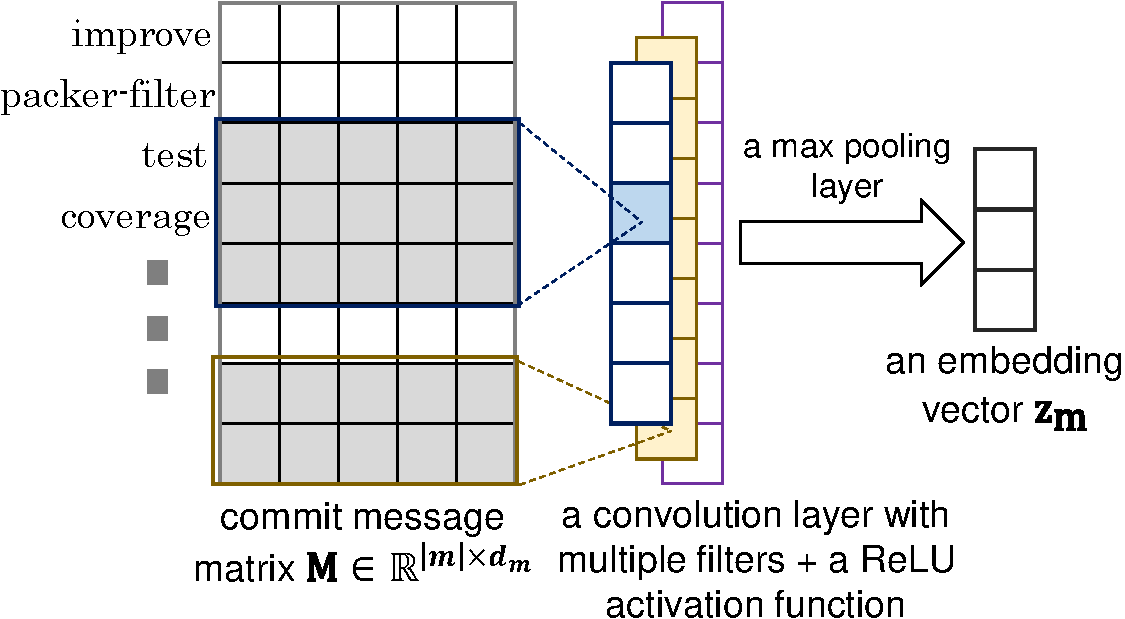
\includegraphics[scale=0.4]{figs/msg.pdf}
\caption{A convolutional network architecture for commit message.}
\label{fig:msg}
\end{figure}
The underlying deep neural network for commit message is a Convolutional Neural Network (CNN). CNN firstly used to automatically learn the salient features in the images from raw pixel values~\cite{krizhevsky2012imagenet}. However, CNN has been also used a lot and showed extraordinary successes in Natural Language Processing (NLP)~\cite{kim2014convolutional, dos2014deep, kalchbrenner2014convolutional, zhang2015character, johnson2014effective}. The architecture of CNN allowed it to extract the structural information features from raw text data of word embedding. Figure~\ref{fig:msg} presents an architecture of CNN for commit message. The architecture includes a convolutional layer with multiple filters and a nonlinear activation function (i.e., RELU). We briefly explain it in the following paragraphs. 

Given a commit message $\textbf{m}$ which is essentially a sequence of words $[w_1, \dots, w_{|m|}]$. We aim to obtains its matrix representation $\textbf{m} \rightarrow \textbf{M} \in \mathbb{R}^{|m| \times d_m}$, where the matrix $\textbf{M}$ comprises a set of words $w_i \rightarrow W_i$, $i = 1, \dots, |m|$ in the given commit message. Each word $w_i$ now is represented by an embedding vector, i.e., $W_i \in \mathbb{R}^{d_m}$, where $d_m$ is a $d_m$-dimensional vector of a word appearing in the commit message. 

Following the previous works~\cite{kim2014convolutional, zhang2015character}, the $d_m$-dimensional representing an embedding vector extracted from an embedding matrix which is randomly initialized and jointly learned with the CNN model. In our paper, the embedding matrix of commit message is randomly initialized and learned during the training process. Hence, the matrix representation $\textbf{M}$ of the commit message $\textbf{m}$ with a sequence of $|m|$ words can be represented as follows:
\begin{equation}
\label{eq:representation_msg}
    \textbf{M} = [W_1, \dots, W_{|m|}]
\end{equation}
For the purpose of parallelization, all commit messages are padded or truncated to the same length $|m|$. 

To extract the commit message's salient features, a filter $f \in \mathbb{R}^{k \times {d_m}}$, followed by a non-linear activation function $\alpha (.)$, is applied to a window of $k$ words to produce a new feature as follows:
\begin{equation}
\label{eq:filter_msg}
    c_i = \alpha(f * M_{i:i+k-1} + b_i)
\end{equation}
where $*$ is a sum of element-wise product, and $b_i \in \mathbb{R}$ is the bias value. In our paper, we choose the rectified linear unit (RELU) as our activation function since it achieved a better performance compared to other activation functions~\cite{nair2010rectified, dahl2013improving, he2016deep}. The filter $f$ is applied to every $k$-words of the commit message, these outputs of this process are then concatenated to product output vector $\textbf{c}$ such that:
\begin{equation}
\label{eq:output_ftr_msg}
\textbf{c} = [c_1, \dots, c_{|m| - k + 1}]
\end{equation}

By applying the filter $f$ on every $k$-words of the commit message, the CNN is able to exploit the semantic information of its input. In practice, the CNN model may include multiple filters with different $k$. These hyperparameters need to be set by the user before starting the training process. To characterize the commit message, we apply a max pooling operation~\cite{lecun2015deep} over the output vector $\textbf{c}$ to obtain the highest value as follows: 

\begin{equation}
\label{eq:max_pooling_msg}
\underset{1 \leq i \leq |m| - k + 1}{max} c_i
\end{equation}

The results of the max pooling operation from each filter are then used to form an embedding vector (i.e., $\textbf{z}_\textbf{m}$) of the commit message (see Figure~\ref{fig:overview}). 

\subsection{Convolutional Network Architecture for Code Changes}
\label{sec:cnn_code}

\begin{figure*}
	\center
	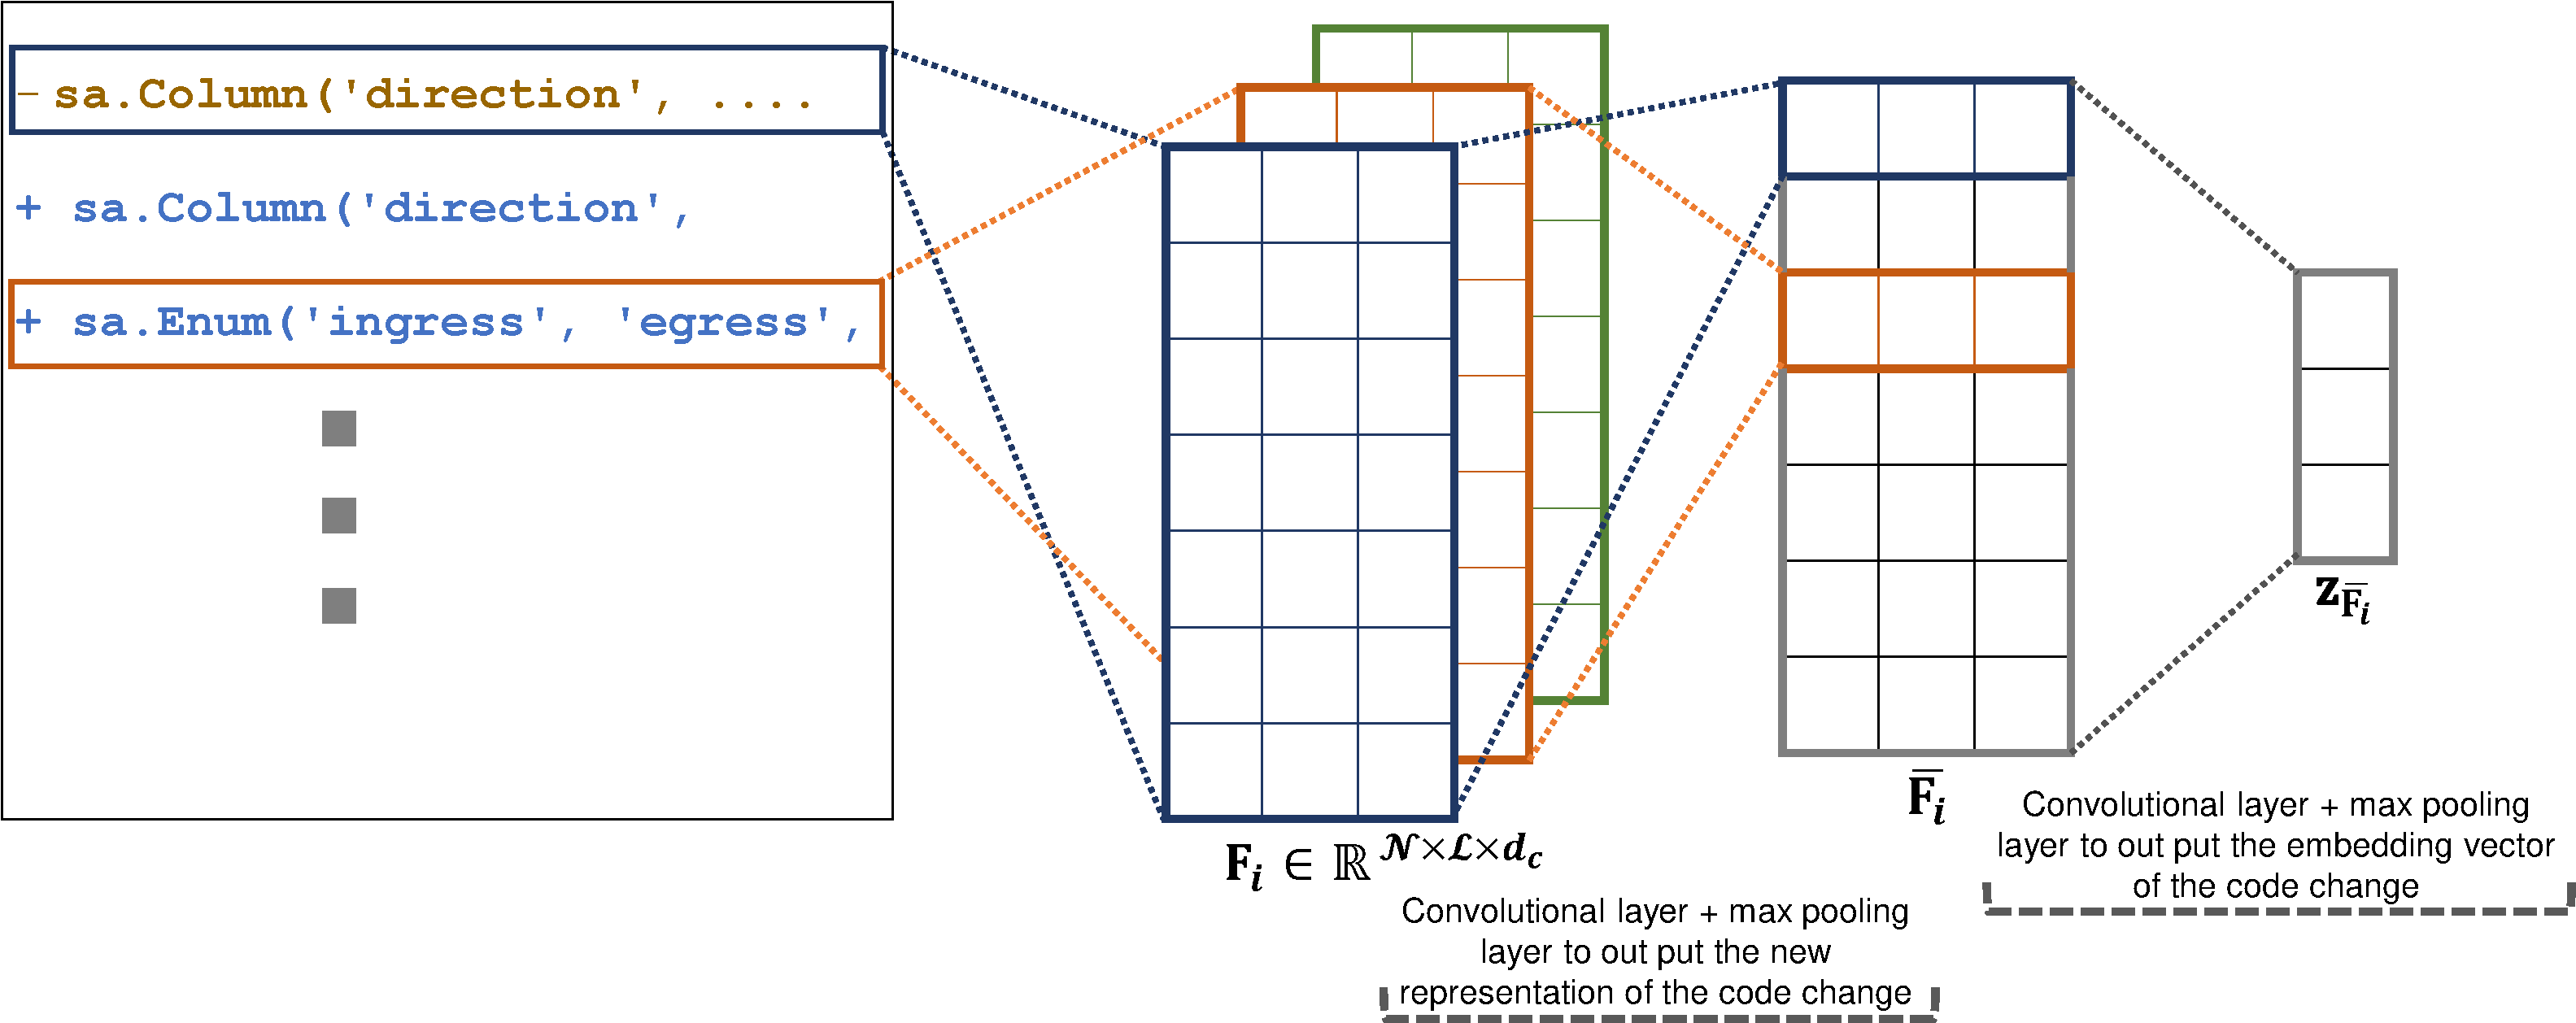
\includegraphics[scale=0.25]{figs/code_framework.pdf}
	\caption{The overall structure of convolutional neural network for each change file in code change. The first convolutional and pooling layers use to learn the semantic features of each added or removed code line based on the words within the added or removed line, and the subsequent convolutional and pooling layers aim to learn the interactions between added or removed code line with respect to the code change structure. The output of the convolutional neural network is the embedding vector $\textbf{z}_{\overline{\textbf{F}}_{i}}$ representing the salient features of the each change file.}
	\label{fig:code}
\end{figure*}

In this section, we focus on building convolutional networks for code changes to solve the just-in-time defect prediction problem. 
Code change, although it can be viewed as a sequence of words, differs from natural language mainly because of its structure. The natural language carries sequences of words, and the semantics of the natural language can be inferred from a bag of words~\cite{ng1997corpus}. On the other hand, the code change includes a change in different files and different kinds of changes (removals or additions) for each file. Hence, to extract salient features from the code changes, the convolutional networks should obey the code changes structure. 
Based on the aforementioned considerations, we propose novel neural networks for extracting silent features from code changes based on convolutional neural networks. 

Given a code change $\mathcal{C}$ including a change in different source code files $[\text{F}_1, \dots, \text{F}_n]$, where $n$ is a number of files in the code change, we aim to extract salient features for each different file $\text{F}_i$. The salient features of each file are then concatenated to each other to represent the features for the given code change. In the rest of this section, we explain how the convolutional networks can extract the salient features for each file in the code change and how these salient features are concatenated. 

Suppose $\text{F}_i$ represents a change in each different file, $\text{F}_i$ contains a number of lines (removals or additions) in a code change file. We also have a sequence of words in each line in $\text{F}_i$. Similar to the section~\ref{sec:cnn_msg}, we first aim to obtain its matrix representation $\text{F}_i \rightarrow \textbf{\text{F}}_i \in \mathbb{R}^{\mathcal{N} \times \mathcal{L} \times{d_c}}$, where $\mathcal{N}$ is the number of lines in a code change file, $\mathcal{L}$ presents a sequence of words in each line, and $d_c$ is a $d_c$-dimensional vector of a word appearing in the $\text{F}_i$. For the purposed of parallelization, all the source code files are padded or truncated to the same $\mathcal{N}$ and $\mathcal{L}$. 

For each line $\mathcal{N}_i \in \mathbb{R}^{\mathcal{L} \times d_c}$, we follow the convolutional network architecture for commit message described in section~\ref{sec:cnn_msg} to extract its embedding vector, called $\textbf{z}_{\mathcal{N}_i}$. The embedding vector $\textbf{z}_{\mathcal{N}_i}$ aims to learn the salient features or the semantic of a code line based on the words within the code line. These features $\textbf{z}_{\mathcal{N}_i}$ are then stacked to produce the new representation of the code change file $\text{F}_i$ as follows: 
\begin{equation}
\label{eq:concatenate}
\overline{\textbf{F}}_{i} = [\textbf{z}_{\mathcal{N}_1}, \dots, \textbf{z}_{\mathcal{N}_{|\mathcal{N}|}}]
\end{equation}

We again apply the convolutional layer and pooling layer on the new representation of the code change (i.e., $\overline{\textbf{F}}_{i}$) to extract its embedding vector, namely $\textbf{z}_{\overline{\textbf{F}}_{i}}$. The $\textbf{z}_{\overline{\textbf{F}}_{i}}$ aims to learn the salient features or the semantics conveyed by the interactions between added or deleted lines. Figure~\ref{fig:code} presents an overall convolutional network architecture for each change file $F_i$ in code changes. The first convolutional and pooling layers aim to learn a new representation of the file, and the subsequent convolutional and pooling layers aim to extract the salient features from the new representation of the change file. 

For each change file $\text{F}_i \in C$, we build its embedding vector $\textbf{z}_{\overline{\textbf{F}}_{i}}$. These embedding vectors are then concatenated to build a new embedding vector representing the salient features of the code change $C$ as follows: 
\begin{equation}
\label{eq:concatenate_code}
\textbf{z}_C = \textbf{z}_{\overline{\textbf{F}}_{1}} \oplus \dots \oplus \textbf{z}_{\overline{\textbf{F}}_{n}}
\end{equation}
where $\oplus$ is the concatenation operator. 

%For each line $\mathcal{L}_i$, we follow the convolutional networks described in section~\ref{sec:cnn_msg} to extract its features, called $\textbf{z}_{\mathcal{L}_i}$.

\subsection{Feature Combination}
\label{sec:ftr_combine}
\begin{figure}
	\center
	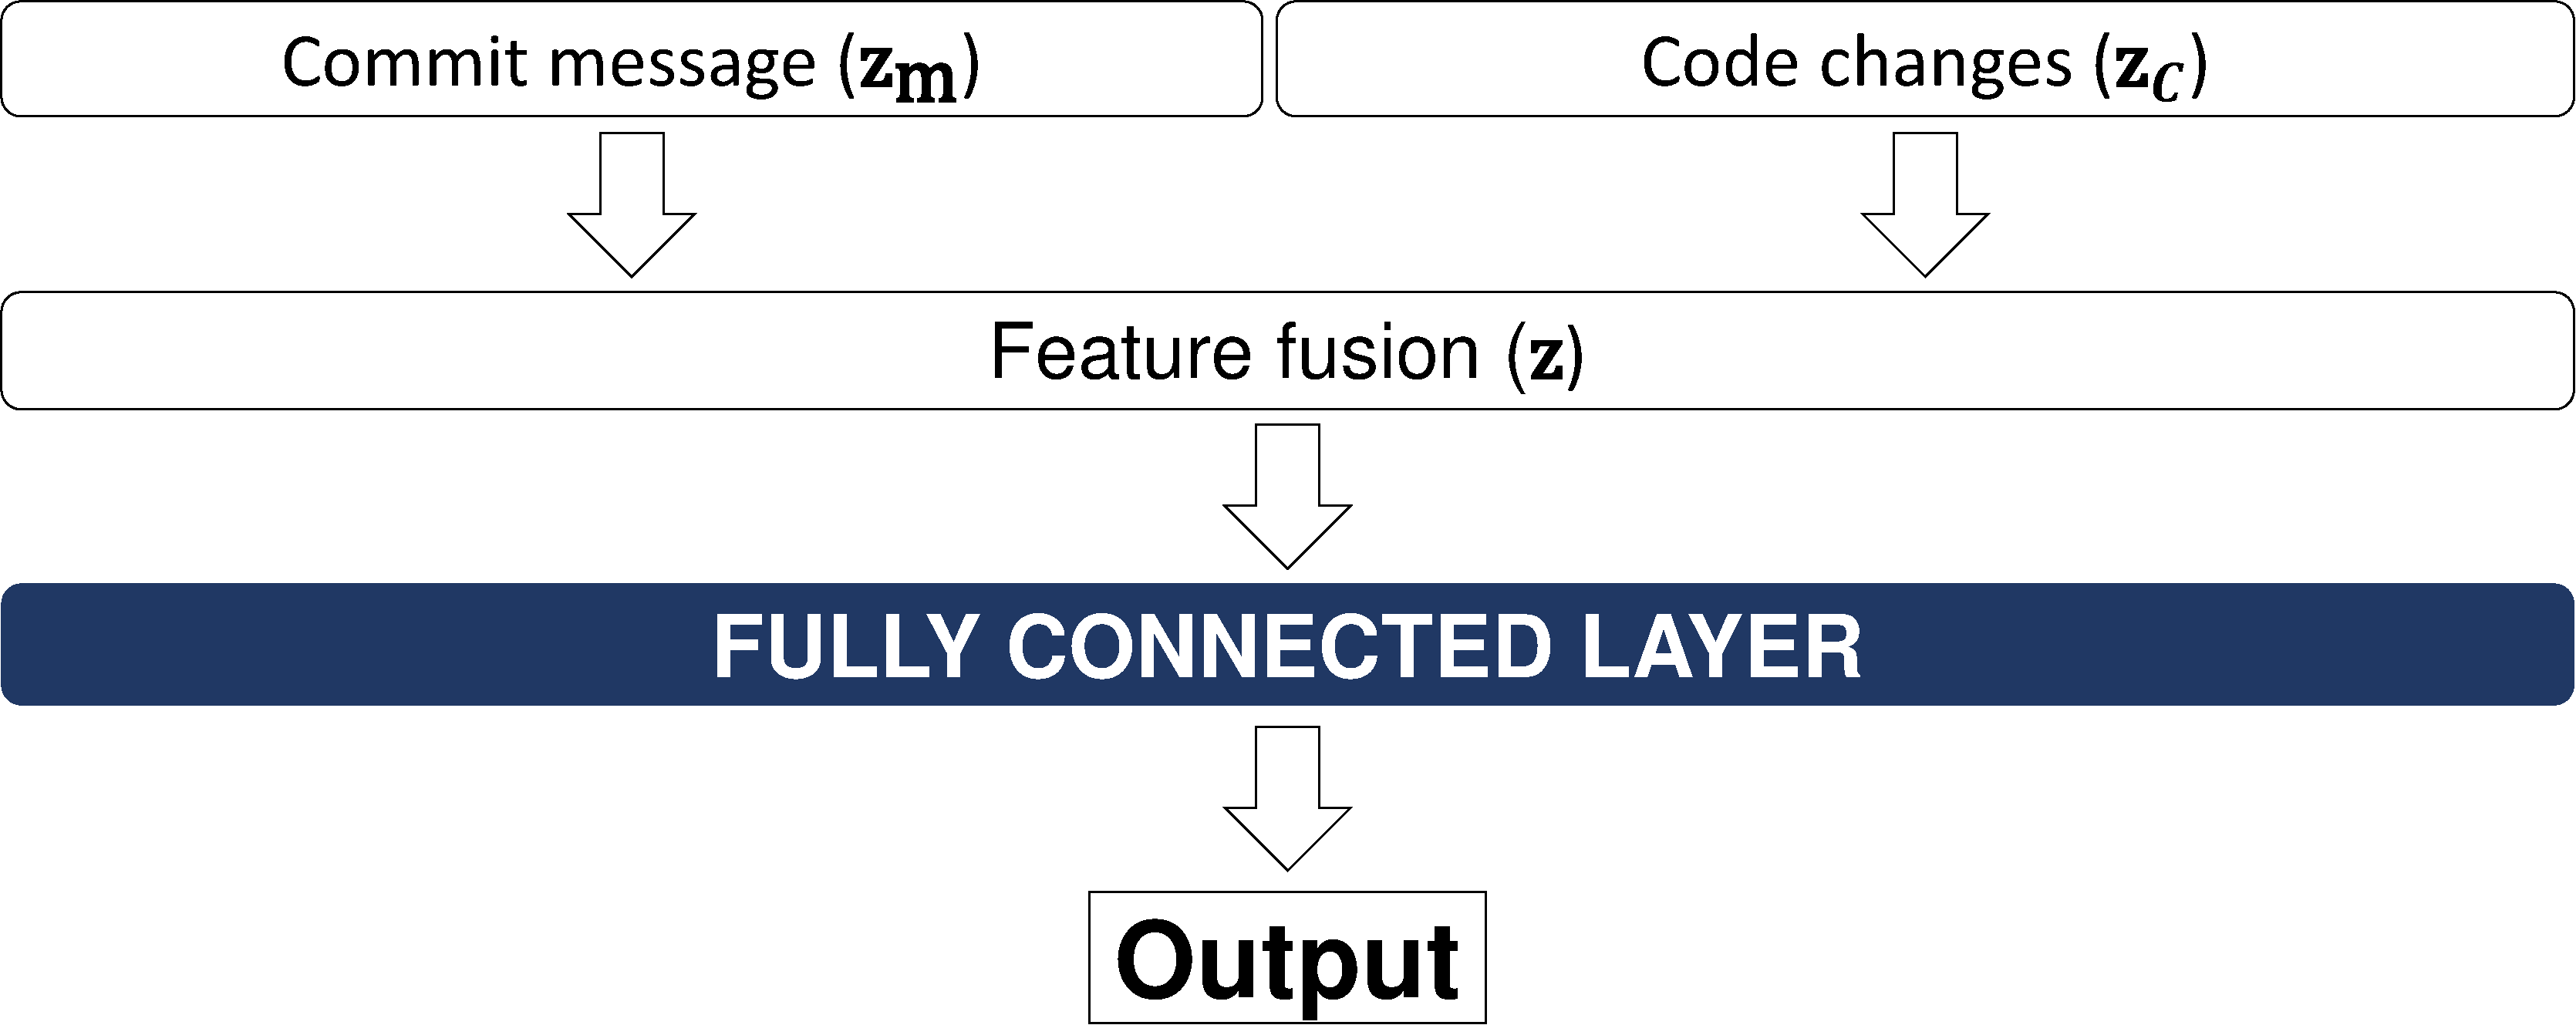
\includegraphics[scale=0.15]{figs/code_msg.pdf}
	\caption{The structure of fully-connected network for feature combination. The embedding vector of commit message $\textbf{z}_\textbf{m}$ and code change $\textbf{z}_C$ are concatenated to generate a single vector (i.e., $\textbf{z}$).}
	\label{fig:code_msg}
\end{figure}

Figure~\ref{fig:code_msg} shows the details of architecture of the feature combination. The inputs of this architecture are the two embedding vectors $\textbf{z}_\textbf{m}$ and $\textbf{z}_C$ which represent the salient features extracted from the commit message and code change, respectively. 

These vectors are then concatenated to generate a unified feature representation, i.e., a new vector ($\textbf{z}$), representing the commit change:
\begin{equation}
\label{eq:commit_code}
\textbf{z} = \textbf{z}_\textbf{m} \oplus \textbf{z}_C
\end{equation}

The new vector then feed into a fully-connected (FC) layer, which outputs a vector $\textbf{h}$ as follows:
\begin{equation}  % \footnotesize
\label{eq:fully_layer}
\textbf{h} = \alpha(\textbf{w}_\textbf{h} \cdot \textbf{z} + b_\textbf{h})
\end{equation}
where $\cdot$ is a dot product, $\textbf{w}_h$ is a weight matrix of the vector $\textbf{h}$ and the FC layer, $b_\textbf{h}$ is the bias value, and $\alpha(\cdot)$ is the RELU activation function. The vector $\textbf{h}$ is passed to an output layer to compute a probability score for a given commit:


Finally, the vector $\mathbf{h}$ is passed to an output layer, which
computes a probability score for a given patch:
\begin{equation}  %\footnotesize
p(y_i=1|x_i) = \frac{1}{1 + \exp({-\textbf{h} \cdot \textbf{w}_\textbf{o})}}
\end{equation}
where $\textbf{w}_\textbf{o}$ is the weight matrix between the FC layer and the output layer.

\subsection{Parameters Learning}
\label{sec:learning_parameters}

In the training process, DeepJIT aims to learn the following parameters: the
word embedding matrices of commit messages and commit code in a given commit, the convolutional layers matrices, the weights and bias of
the fully connected layer and the output layer. 

In the \emph{Just-In-Time} defect prediction, only a few commits contain a buggy code while a large number of commits are clean. Such an imbalance nature increases the difficulty in learning a prediction function~\cite{chawla2004special}. Inspired by~\cite{zhou2006training, kukar1998cost}, we propose an unequal misclassification loss function which helps to reduce the negative influence of the imbalanced data. 

Let $\textbf{w}_\textbf{n}$ and $\textbf{w}_\textbf{p}$ are the cost of incorrectly associating a commit change and the cost of missing a buggy commit change, respectively. The parameters of DeepJIT can be learned by minimizing the following objective function:
\begin{equation} %\footnotesize
\label{eq:cost}
\begin{split}
\mathcal{O} &= -\log\left( \prod_{i=1}^{} p(y_i|x_i) \right) + \frac{\lambda}{2} \|\theta\|_{2}^{2} \\
&= -\sum_{i=1}^{} [ \textbf{w}_\textbf{n} (1 - y_i) \log(1 - p(y_i|x_i)) \\ 
&+ \textbf{w}_\textbf{p} y_i \log (p(y_i|x_i)) ] + \frac{\lambda}{2} \|\theta\|_{2}^{2}
\end{split}
\end{equation}
where $p(y_i|x_i)$ is the probability score from the output layer and $\theta$ contains all parameters our model. The term $\frac{\lambda}{2} \|\theta\|_{2}^{2}$ is used to mitigate data overfitting in training deep neural networks~\cite{caruana2001overfitting}. We also apply the dropout technique~\cite{srivastava2014dropout} to improve the robustness of our model. 

We choose Adam~\cite{kingma2014adam}, which is a variant of stochastic gradient descent (SGD)~\cite{bottou2010large}, to minimize the objective function in the equation~\ref{eq:cost}. We choose Adam due to its computational efficiency and low memory requirements compared to other optimization techniques~\cite{kingma2014adam, anthimopoulos2016lung, arora2018optimization}. To efficiently compute the gradients in linear time (with respect to the neural network size), we use backpropagation~\cite{hagan1994training}, which is a simple implementation of the chain rule of partial derivatives.

\section{Experiments}
\label{sec:exp}
In this section, we first describe the dataset used in our paper. We then introduce all baselines, evaluation metric, and setting. Finally, we present our research questions and results.

\subsection{Dataset}
\label{sec:dataset}
\cmt{TODO: add the information about the dataset}

\subsection{Baseline}
\label{sec:baseline}
We compared DeepJIT with two other state-of-the-art baselines in the \emph{Just-In-Time} (JIT) defect prediction:
\begin{itemize}
\item JIT: The method for identifying fix-inducing code changes was proposed by McIntosh and Kamei~\cite{mcintosh2018fix}. The method used a nonlinear variant of multiple regression modeling~\cite{fox1997applied} to build a classification model for automatically identifying defects in commits. The set of code features, using six families of code change properties, were primarily derived from prior studies~\cite{Kamei:2013:LES, Kim:2008:CSC, Kononenko:2015, Mockus2000}. These properties were: the magnitude of change, the dispersion of the changes, the defect proneness of prior changes, the experience of the author, the code reviewers, and the degree of participation in the code review. 
\item DBN-JIT: The method adopted Deep Belief Network (DBN)~\cite{hinton2006reducing}, one of the state-of-the-art deep learning approaches, to generate a more expressive feature set from the initial feature set~\cite{Yang:2015:DLJ}. The generated feature set, a complicated nonlinear combination of the initial features, was put to a machine learning classifier~\cite{nasrabadi2007pattern} to predict defects in commits. 
\end{itemize}

\subsection{Training and hyperparameters}
\label{sec:training_parameters}
For the size of the convolutional filters, we choose 64. The size of DeepJIT's fully-connected layer described in Section~\ref{sec:ftr_combine} is set to 512. The word vectors dimension of the commit message ($d_m$) and code changes ($d_c$) are set to 64. We train DeepJIT using Adam~\cite{kingma2014adam} with shuffled mini-batches.  The batch size is set to 32. We train DeepJIT for 100 epochs. We also apply the early stopping strategy~\cite{prechelt1998automatic, caruana2001overfitting} to avoid overfitting problem during the training process. Typically, we stop the training if the value of the objective function (see Equation~\ref{eq:cost}) has been no update in the last 5 epochs. All these hyperparameters in our paper are widely used in the deep learning community~\cite{severyn2015learning, huo2016learning, huo2017enhancing, hinton2012improving}. 
 
\subsection{Evaluation Metric}
\label{sec:metric}
To evaluate the accuracy of \emph{Just-In-Time} (JIT) models, we calculate  threshold-independent measures of model performance. Since our dataset is imbalanced data, we avoid using threshold-dependent measures (i.e., precision, recall, or F1) since these measures strongly depend on arbitraily thresholds~\cite{nguyen2009learning, gu2008data}. Following the previous work~\cite{mcintosh2018fix},  we use the Area Under the receiver operator characteristics
Curve (AUC) to measure the power of models' discriminatory, i.e., their ability to differentiate between defects or clean commits. AUC computes the area under the curve ploting the true 

We
avoid threshold-dependent measures like precision and recall, which depend on arbitrarily thresholds and are sensitive to imbalanced data.
The Area Under the receiver operator characteristics
Curve (AUC) is a measure of a model’s discriminatory power,
i.e., its ability to differentiate between fix-inducing and clean
changes. AUC is computed by measuring the area under
the curve that plots the true positive rate against the false
positive rate, while varying the threshold that is used to
determine if a change is classified as fix-inducing or not.
Values of AUC range between 0 (worst discrimination), 0.5
(random guessing), and 1 (perfect discrimination).


\subsection{Research Questions and Results}
\label{sec:rq_results}

\noindent \textbf{RQ1: How effective is our proposed deep learning model compared to the state-of-the-art baseline?}

\begin{figure}
\center
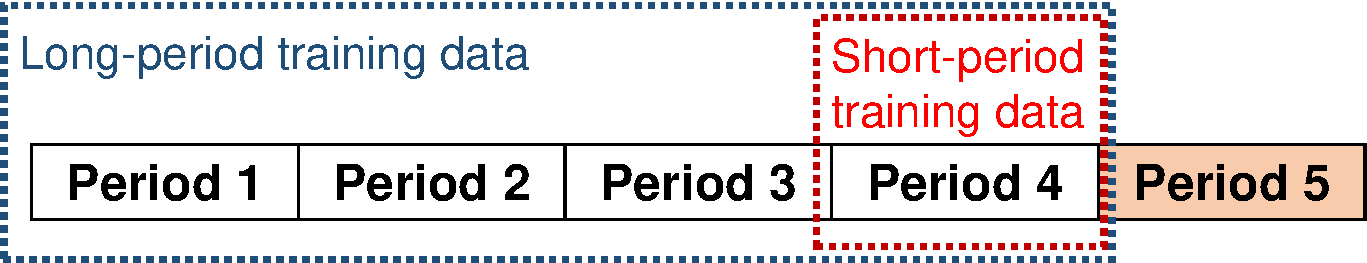
\includegraphics[scale=0.36]{figs/split.pdf}
\caption{An example of choosing the data for training proposed model. The last period will be used as testing data.}
\label{fig:splitting}
\end{figure}

\begin{table*}[t!]
  \centering
  \caption{The AUC results of DeepJIT vs. with other baselines in three settings: short-period, long-period, and random}
    \begin{tabular}{|l|c|c|c|c|c|c|}
    \hline
    \multirow{2}[4]{*}{} & \multicolumn{3}{c|}{QT} & \multicolumn{3}{c|}{OPENSTACK} \\
\cline{2-7}          & \multicolumn{1}{l|}{Short-Period} & \multicolumn{1}{l|}{Long-period} & \multicolumn{1}{l|}{Random} & \multicolumn{1}{l|}{Short-Period} & \multicolumn{1}{l|}{Long-period} & \multicolumn{1}{l|}{Random} \\
    \hline
    \hline
    JIT   & 0.703 & 0.702 & 0.701 & 0.711 & 0.706 & 0.691 \\
    \hline
    DBNJIT & 0.714 & 0.708 & 0.705 & 0.716 & 0.712 & 0.694 \\
    \hline
    DeepJIT & \textbf{0.764} & \textbf{0.765} & \textbf{0.768} & \textbf{0.781} & \textbf{0.771} & \textbf{0.751} \\
    \hline
    \end{tabular}%
  \label{tab:results}%
\end{table*}%

\noindent \textbf{RQ2: Does the proposed model benefit both commit message and the code changes?}

\begin{table*}[t!]
  \centering
  \caption{Contribution of feature components in DeepJIT}
    \begin{tabular}{|l|c|c|c|c|c|c|}
    \hline
    \multirow{2}[4]{*}{} & \multicolumn{3}{c|}{QT} & \multicolumn{3}{c|}{OPENSTACK} \\
\cline{2-7}          & \multicolumn{1}{l|}{Short-Period} & \multicolumn{1}{l|}{Long-period} & \multicolumn{1}{l|}{Random} & \multicolumn{1}{l|}{Short-Period} & \multicolumn{1}{l|}{Long-period} & \multicolumn{1}{l|}{Random} \\
    \hline
    \hline
    DeepJIT-Msg & 0.609 & 0.638 & 0.641 & 0.583 & 0.659 & 0.689 \\
    \hline
    DeepJIT-Code & 0.734 & 0.727 & 0.738 & 0.769 & 0.738 & 0.729 \\
    \hline
    DeepJIT & \textbf{0.764} & \textbf{0.765} & \textbf{0.768} & \textbf{0.781} & \textbf{0.771} \\
    \hline
    \end{tabular}%
  \label{tab:variants}%
\end{table*}%

\noindent \textbf{RQ3: Does the proposed model benefit from the manually extracted code changes features?}

\begin{table*}[t!]
  \centering
  \caption{Combination of DeepJIT with JIT's features}
    \begin{tabular}{|l|c|c|c|c|c|c|}
    \hline
    \multirow{2}[4]{*}{} & \multicolumn{3}{c|}{QT} & \multicolumn{3}{c|}{OPENSTACK} \\
\cline{2-7}          & Short-Period & Long-period & Random & Short-Period & Long-period & Random \\
    \hline
    \hline
    DeepJIT & 0.764 & 0.765 & 0.768 & 0.781 & 0.771 & 0.751 \\
    \hline
    DeepJIT-Combined & \textbf{0.788} & \textbf{0.786} & \textbf{0.779} & \textbf{0.814} & \textbf{0.799} & \text{0.760} \\
    \hline
    \end{tabular}%
  \label{tab:combined}%
\end{table*}%

\noindent \textbf{RQ4: How are the time costs of the proposed model?}



\section{Threats to Validity}
\label{sec:threat}
\section{Related Work}
\label{sec:related}
\subsection{JIT Defect Prediction}
Some previous studies focus on change-level defect prediction (i.e., JIT defect prediction). For example, Mockus and Weiss~\cite{Mockus2000} predict commits as being buggy or not in an industrial project. They use metric-based features, such as the number of subsystems touched, the number of files modified, the number of lines of added code, and the number of modification requests. Motivated by their previous work, Kamei et al.~\cite{Kamei:2013:LES} built upon the set of code change features, reporting that the addition of a variety of features that were extracted from the Version Control System (VCS) and the Issue Tracking System (ITS) helped to improve the prediction accuracy. They conduct an empirical study of the effectiveness of JIT defect prediction on a set of six open source and five commercial projects and also evaluate their findings when considering the effort required to review the changes.

Aversano \emph{et al.}~\cite{Aversano2007} and Kim \emph{et al.}~\cite{Kim2008} use source code change logs to predict commits as being buggy or not. For example, Kim \emph{et al.}~\cite{Kim2008} used the identifiers in added and deleted source code and the words in change logs. The experimental results on the datasets collected from 12 open source software projects show that the proposed approach achieve 78 percent accuracy and a 60 percent recall.

Kononenko et al.~\cite{Kononenko:2015} found that the addition of code change properties that were extracted from code review databases contributed a significant amount of explanatory power to JIT models. McIntosh and Kamei also 
%\cmt{TODO: update here} 
%The importance of impactful families of code change properties like Size and Review are consistently under/overestimated in the studied systems.

Comparing with these previous studies, we introduce the JIT defect prediction model (DeepJIT) that learn a deep representation of commits and compare the prediction performance of DeepJIT with other JIT models on the dataset including code change properties that are extracted from code review databases. We extended the datasets that McIntosh and Kamei used to analyze~\footnote{\url{https://github.com/software-rebels/JITMovingTarget}} by adding commit messages and code changes. 

\subsection{Deep Learning Models in Defect Prediction}

%Xin Xia's group

%Lin Tang's group

%Say the difference between them and us.
\section{Conclusion}
\label{sec:conclusion}



\bibliographystyle{ACM-Reference-Format}
\bibliography{bib,JIT,TSE_ChangeRisk,security}

\end{document}
